\documentclass[professionalfont]{beamer}
%\usecolortheme{default}
\usetheme{Madrid}
\usepackage{subcaption}
\usepackage{caption}
\theoremstyle{definition}
\usepackage{tikz}


\title{\textbf{Lieb-Schultz-Mattis Theorem for Open Quantum Systems}}

\author{Chen-Chih Wang}
\institute{Department of Physics, National Tsing Hua University}
\date{April 18, 2024}

\newcommand{\pdiff}[2]{\frac{\partial #1}{\partial #2}}
\newcommand{\diff}[2]{\frac{\mathrm{d} #1}{\mathrm{d} #2}}
\newcommand{\dif}[1]{\frac{\mathrm{d}}{\mathrm{d} #1}}
\newcommand{\lr}[1]{\left(#1\right)}
\newcommand{\anglelr}[1]{\langle#1\rangle}
\newcommand{\lrm}[1]{\left[#1\right]}
\newcommand{\lrg}[1]{\left\{#1\right\}}
\newcommand{\lran}[1]{\left\langle #1 \right\rangle}
\newcommand{\lra}[1]{\left|#1\right|}
\newcommand{\ket}[1]{\left| #1 \right\rangle}
\newcommand{\bra}[1]{\left\langle #1 \right|}
\newcommand{\braket}[2]{\left\langle #1 \right|\left. #2\right\rangle}
\newcommand{\mrm}[1]{\mathrm{#1}}
\newcommand{\bo}[1]{\mathbf{#1}}
\newcommand{\gk}{\gamma_{\mathbf{k}}}
\newcommand{\uk}{u_{\mathbf{k}}}
\newcommand{\vk}{v_{\mathbf{k}}}
\newcommand{\vkp}{v_{\mathbf{k}'}}
\newcommand{\here}{$\blacktriangleright$}

%\setbeamercolor{frametitle}{fg=black,bg=blue}
%\setbeamertemplate{frametitle}[default][left]
%\setbeamerfont{frametitle}{size=\huge}
%\setbeamerfont{block title}{size=\Large}

%%%%%%%%%%%%%%%%%%%%%%%%%%%%%%%%%%%%%%%%%%%%%%%%

\begin{document}
\begin{frame}
    \titlepage
\end{frame}

%%%%%%%%%%%%%%%%%%  content  %%%%%%%%%%%%%%%%%%%
\begin{frame}{Content}
   \tableofcontents
\end{frame}

%%%%%%%%%%%%%%%%%%%%%%%%%%%%%%%%%%%%%%%%%%%%%%%%
\begin{frame}{Literature}
\section{Literature}
    \begin{enumerate}
        \item Yi-Neng Zhou, Xingyu Li, Hui Zhai, Chengshu Li, and Yingfei Gu, \textit{Reviving the Lieb-Schultz-Mattis Theorem in Open Quantum Systems}, arXiv:2310.01475
        \item Kohei Kawabata, Ramanjit Sohal, and Shinsei Ryu, \emph{Lieb-Shultz-Mattis Theorem in Open Quantum Systems}, \\ \emph{Phys. Rev. Lett.} \textbf{132}, 070402 (2024)
    \end{enumerate}
\end{frame}
%%%%%%%%%%%%%%%%%%%%%%%%%%%%%%%%%%%%%%%%%%%%%%%%
\begin{frame}{Introduction}
\section{Introduction}
\begin{theorem}[Lieb-Schultz-Mattis]
     A one-dimensional periodic chain of length $L$, with half-integer spin per unit cell, has an excitation gap bounded by $\mrm{const.}/L$.
\end{theorem}
So there are three possible scenarios for 1D spin systems:
\begin{enumerate}
    \item Gapless spectrum
    \item Gapped spectrum with spontaneous symmetry breaking
    \item Gapped spectrum with ground state degeneracy 
\end{enumerate}
\textbf{LSM theorem provides the restrictions of 1D quantum systems. }
\end{frame}
%%%%%%%%%%%%%%%%%%%%%%%%%%%%%%%%%%%%%%%%%%%%%%%%
\begin{frame}{Introduction}
    Essence of LSM theorem
    \begin{enumerate}
        \item Define the twist operator 
        \[\hat{U}_{\mrm{twist}}:= \mrm{exp}\lr{i\frac{2\pi}{L}\sum_{j}j\hat{S}_j}\]
        to construct a state $\ket{\psi'}=\hat{U}_{\mrm{twist}}\ket{\psi}$ such that $\braket{\psi}{\psi'} = 0$.
        \item The eigenvalue of $\ket{\psi'}$ is either the ground state energy (ground state degeneracy) or the energy of the first excited state.
        \item For spin-N, such a statement fails (since $[\hat{T},\hat{U}_{\mrm{twist}}]=0$), leads to the possibility for gap opening (Haldane gap).
    \end{enumerate}
\end{frame}
%%%%%%%%%%%%%%%%%%%%%%%%%%%%%%%%%%%%%%%%%%%%%%%%
\begin{frame}{Introduction}
    \textbf{MOTIVATION}: The discussion by LSM is based on a isolated system. Then \textbf{how about the open quantum systems?}

    \vspace{0.3cm}

    In open quantum systems, \textbf{energy spectrum is no longer well-defined}. Physicists need to find a \textbf{new theoretical framework} and the \textbf{new quantity} playing the role in the open quantum systems as the spectral gap did in the original one.
\end{frame}
%%%%%%%%%%%%%%%%%%%%%%%%%%%%%%%%%%%%%%%%%%%%%%%%
\begin{frame}
\centering
\section{Literature 1}
{\Huge Literature 1}

{\Large arXiv:2310.01475}
    
\end{frame}
%%%%%%%%%%%%%%%%%%%%%%%%%%%%%%%%%%%%%%%%%%%%%%%%
\begin{frame}{Entanglement Spectrum}
\subsection{Entanglement Spectrum}
\begin{definition}[Entanglement Hamiltonian]
    \[\hat{\rho}_s = e^{-\hat{K}}\]
    where $\hat{\rho}_s$ is the reduced density matrix of the system. $\hat{K}$ is the \textit{entanglement Hamiltonian}, whose spectrum is called the \textit{entanglement spectrum}.
\end{definition}

\begin{figure}[H]
    \centering
    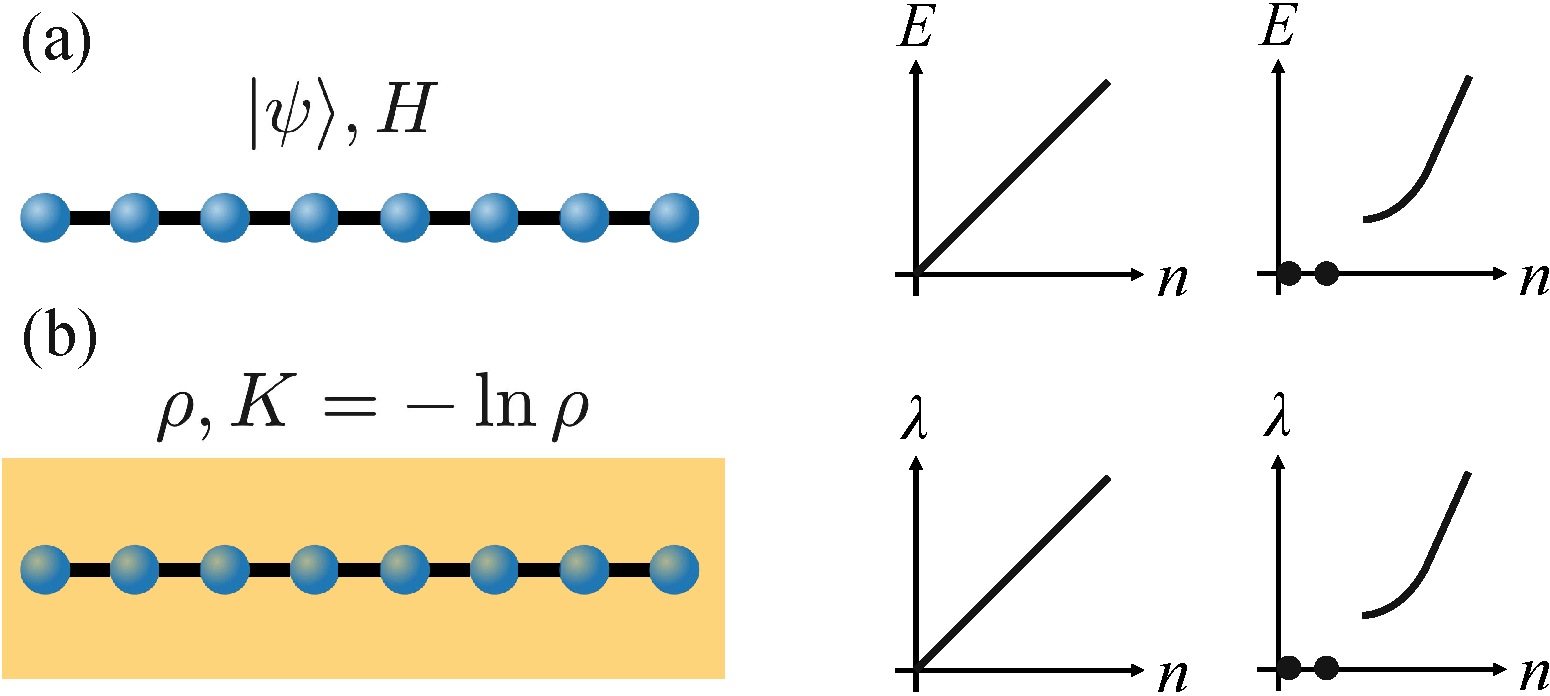
\includegraphics[width = 0.6\textwidth]{entanglement spectrum.pdf}
    \caption{The entanglement spectrum has the similar behaviour to the energy spectrum.}
    \label{entanglement spectrum.f}
\end{figure}
\end{frame}
%%%%%%%%%%%%%%%%%%%%%%%%%%%%%%%%%%%%%%%%%%%%%%%%
\begin{frame}{Entanlgment LSM Theorem}
%\subsection{Entanglement LSM Theorem}
    \begin{theorem}[Entanglement LSM]
        The entanglement spectrum is gapless or has the ground state degeneracy if
        \begin{itemize}
            \item Half-integer representation (ex: spin $S$ or filling factor $\nu$)
            \item Onsite rotational symmetry is preserved.
            \item Short-range correlation behaviour: $\anglelr{S^z_iS^s_j}\sim e^{-|i-j|/\xi}$
        \end{itemize}
    \end{theorem}
    The \textbf{short-range correlation behaviour} is crucial in the latter discussion. Such a phenomenon is caused by the coupling to the environment.
    \begin{enumerate}
        \item $\xi\sim1/\Delta$. The system gap $\Delta$ is opened by the coupling to the bath.
        \item $\xi\sim1/T$. Due to the thermalization.
    \end{enumerate}
\end{frame}
%%%%%%%%%%%%%%%%%%%%%%%%%%%%%%%%%%%%%%%%%%%%%%%%
\begin{frame}{Entanglement LSM Theorem (Theoretical Intuition)}
\textbf{Example}: Coupling between two spin chains. Spin chain $a$ is the system and $b$ is the bath (environment).

\begin{equation*}
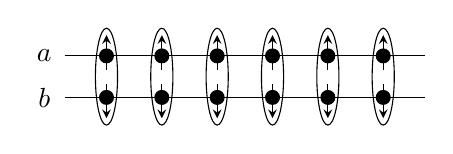
\begin{tikzpicture}[scale=0.5,baseline={([yshift=-7pt]current bounding box.center)}]
\filldraw[fill=black] (0pt,0pt) circle (5pt);
\draw[->,>=stealth] (0pt,-10pt) -- (0pt,15pt);
\filldraw[fill=black] (0pt,-30pt) circle (5pt);
\draw[->,>=stealth] (0pt,-20pt) -- (0pt,-45pt);
\draw (0pt,-15pt) ellipse (8pt and 35pt);

\filldraw[fill=black] (40pt,0pt) circle (5pt);
\draw[->,>=stealth] (40pt,-10pt) -- (40pt,15pt);
\filldraw[fill=black] (40pt,-30pt) circle (5pt);
\draw[->,>=stealth] (40pt,-20pt) -- (40pt,-45pt);
\draw (40pt,-15pt) ellipse (8pt and 35pt);

\filldraw[fill=black] (80pt,0pt) circle (5pt);
\draw[->,>=stealth] (80pt,-10pt) -- (80pt,15pt);
\filldraw[fill=black] (80pt,-30pt) circle (5pt);
\draw[->,>=stealth] (80pt,-20pt) -- (80pt,-45pt);
\draw (80pt,-15pt) ellipse (8pt and 35pt);

\filldraw[fill=black] (120pt,0pt) circle (5pt);
\draw[->,>=stealth] (120pt,-10pt) -- (120pt,15pt);
\filldraw[fill=black] (120pt,-30pt) circle (5pt);
\draw[->,>=stealth] (120pt,-20pt) -- (120pt,-45pt);
\draw (120pt,-15pt) ellipse (8pt and 35pt);

\filldraw[fill=black] (160pt,0pt) circle (5pt);
\draw[->,>=stealth] (160pt,-10pt) -- (160pt,15pt);
\filldraw[fill=black] (160pt,-30pt) circle (5pt);
\draw[->,>=stealth] (160pt,-20pt) -- (160pt,-45pt);
\draw (160pt,-15pt) ellipse (8pt and 35pt);

\filldraw[fill=black] (200pt,0pt) circle (5pt);
\draw[->,>=stealth] (200pt,-10pt) -- (200pt,15pt);
\filldraw[fill=black] (200pt,-30pt) circle (5pt);
\draw[->,>=stealth] (200pt,-20pt) -- (200pt,-45pt);
\draw (200pt,-15pt) ellipse (8pt and 35pt);

\draw (-30pt,0pt) -- (230pt,0pt);
\draw (-30pt,-30pt) -- (230pt,-30pt);
\node at (-45pt,0pt) {$a$};
\node at (-45pt,-30pt) {$b$};
\end{tikzpicture}
\end{equation*}

\[\hat{H} = \lr{J\sum_{i}\hat{\bo{S}}_{i,a}\cdot\hat{\bo{S}}_{i+1,a} + J\sum_{i}\hat{\bo{S}}_{i,b}\cdot\hat{\bo{S}}_{i+1,b}} + \Delta\sum_{i}\hat{\bo{S}}_{i,a}\cdot\hat{\bo{S}}_{i,b}\]

\[\ket{0}=\frac{1}{2^{L/2}}\bigotimes_{i=1}^{L}\lr{\ket{\uparrow}_{i,a}\ket{\downarrow}_{i,b} - \ket{\downarrow}_{i,a}\ket{\uparrow}_{i,b}} = \frac{1}{2^{L/2}}\sum_{n}\ket{n}_a\ket{\bar{n}}_b\]
    
\end{frame}
%%%%%%%%%%%%%%%%%%%%%%%%%%%%%%%%%%%%%%%%%%%%%%%%
\begin{frame}{Entanglement LSM Theorem (Theoretical Intuition)}

{\footnotesize
Apply the perturbation theory,
\[\ket{\psi} \approx \ket{0} - \frac{\hat{H}_a + \hat{H}_b}{2\Delta}\ket{0} \approx e^{-\frac{1}{\Delta}(\hat{H}_a + \hat{H}_b)/2}\ket{0}\]
The reduced density matrix of the system, spin chain $a$, is then
\[\hat{\rho}_s = \mrm{Tr}_b\lr{\ket{\psi}\bra{\psi}} = \frac{1}{2^L}\sum_{n}e^{-2\frac{1}{\Delta}E_n}\ket{n}_a\bra{n}_a = \frac{1}{2^L}e^{2\frac{1}{\Delta}\hat{H}}\]
Based on this, the entanglement Hamiltonian is connected with the Hamiltonian we are familiar with,
\[\hat{K}\sim \frac{1}{\Delta}\hat{H}\]
}
$\blacktriangleright$ The entanglement spectrum satisfies the LSM theorem.


\end{frame}
%%%%%%%%%%%%%%%%%%%%%%%%%%%%%%%%%%%%%%%%%%%%%%%%
\begin{frame}{Locality and Mutual Information}
\subsection{Locality and Mutual Information}

{\Large\textbf{Question}}: An \textbf{information theoretical description }of the \textbf{locality} of the entanglement Hamiltonian.

\vspace{0.3cm}

{\Large\textbf{Goal}}: To show that the spectral gap of $\hat{K}$ vanishes in the $L\to\infty$ limit.

\vspace{0.3cm}

\here \textbf{Mutual Information Function}

\[I(A:B) \equiv S_A + S_B - S_{A\cup B}\]
\begin{align*}
    I(A:C|B) &\equiv  I(A:B\cup C) - I(A:B) \\
    &= I(C:B\cup A) - I(C:B) \\
    &= S_{A\cup B} + S_{C\cup B} - S_B - S_{A\cup B\cup C}
\end{align*}
The conditional mutual information $I(A:C|B)$ measures the information coupling between $A$ and $C$ bridged by $B$.


\end{frame}
%%%%%%%%%%%%%%%%%%%%%%%%%%%%%%%%%%%%%%%%%%%%%%%%
\begin{frame}{Locality and Mutual Information}
\begin{figure}[H]
    \centering
    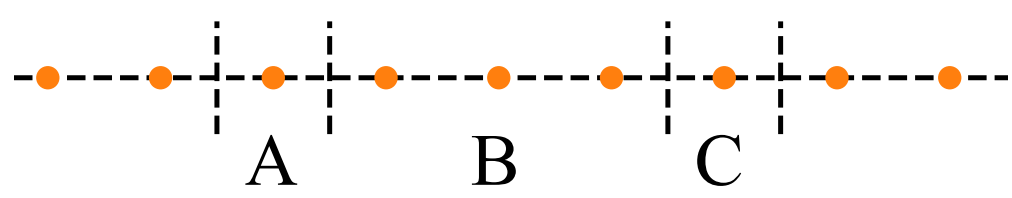
\includegraphics[width = 0.6\textwidth]{ABC.png}
    \caption{The ground state of the system discussed in the literature is a quantum approximate Markov state with $\epsilon\sim e^{-l/\xi}$, where $l$ is the length scale of the bridge subsystem $B$.}
    \label{ABC.e}
\end{figure}
\begin{itemize}
    \item \textbf{Quantum Markov state}: $I(A:C|B) = 0$ 

    Which implies 
    \begin{equation}\label{local.e}
    S_{A\cup B\cup C} = S_{A\cup B} + S_{C\cup B} - S_B
    \end{equation}
    indicating the locality.
    \item \textbf{Quantum approximate Markov state}: $I(A:C|B)<\epsilon\sim e^{-l/\xi}$
\end{itemize}
\end{frame}
%%%%%%%%%%%%%%%%%%%%%%%%%%%%%%%%%%%%%%%%%%%%%%%%
\begin{frame}{Locality and Mutual Information}
\begin{itemize}
    \item[\here] According to the authors, equation    (\ref{local.e}) is equivalent to saying
    \[\hat{K}_{A\cup B\cup C} = \hat{K}_{A\cup B} + \hat{K}_{C\cup B} - \hat{K}_B\]
    That is to say, the \textbf{entanglement Hamiltonian is local}, namely it could be decomposed into a sum of the entanglement Hamiltonian for smaller patches. 

    \item[\here] For quantum approximate Markov states, the entanglement entropy is exponentially local characterized by $e^{-l/\xi}$

    \item[\here] However, \textbf{the statement that the state here is a quantum approximate Markov state has not yet been rigorously proved.} So such a statement is just based on the numerical result.
\end{itemize}


\vspace{0.3cm}


\end{frame}
%%%%%%%%%%%%%%%%%%%%%%%%%%%%%%%%%%%%%%%%%%%%%%%%
\begin{frame}{Numerical Result}
\subsection{Numerical Result}
{\footnotesize\[\hat{H} = J_1\sum_{i=1}^{L}\lr{\hat{\bo{S}}_{i}\cdot \hat{\bo{S}}_{i+1} + \frac{1}{3}\lr{\hat{\bo{S}}_{i}\cdot \hat{\bo{S}}_{i+1}}^2} + J_2\sum_{i=1}^{L}\hat{\bo{S}}_{i,s}\cdot \hat{\bo{S}}_{i,b}\]}
where $\hat{\bo{S}}_{i} = \hat{\bo{S}}_{i,s} + \hat{\bo{S}}_{i,b}$. The system $s$ is a spin-1/2 chain and the bath $b$ is a spin-3/2 chain.
\begin{figure}
    \centering
    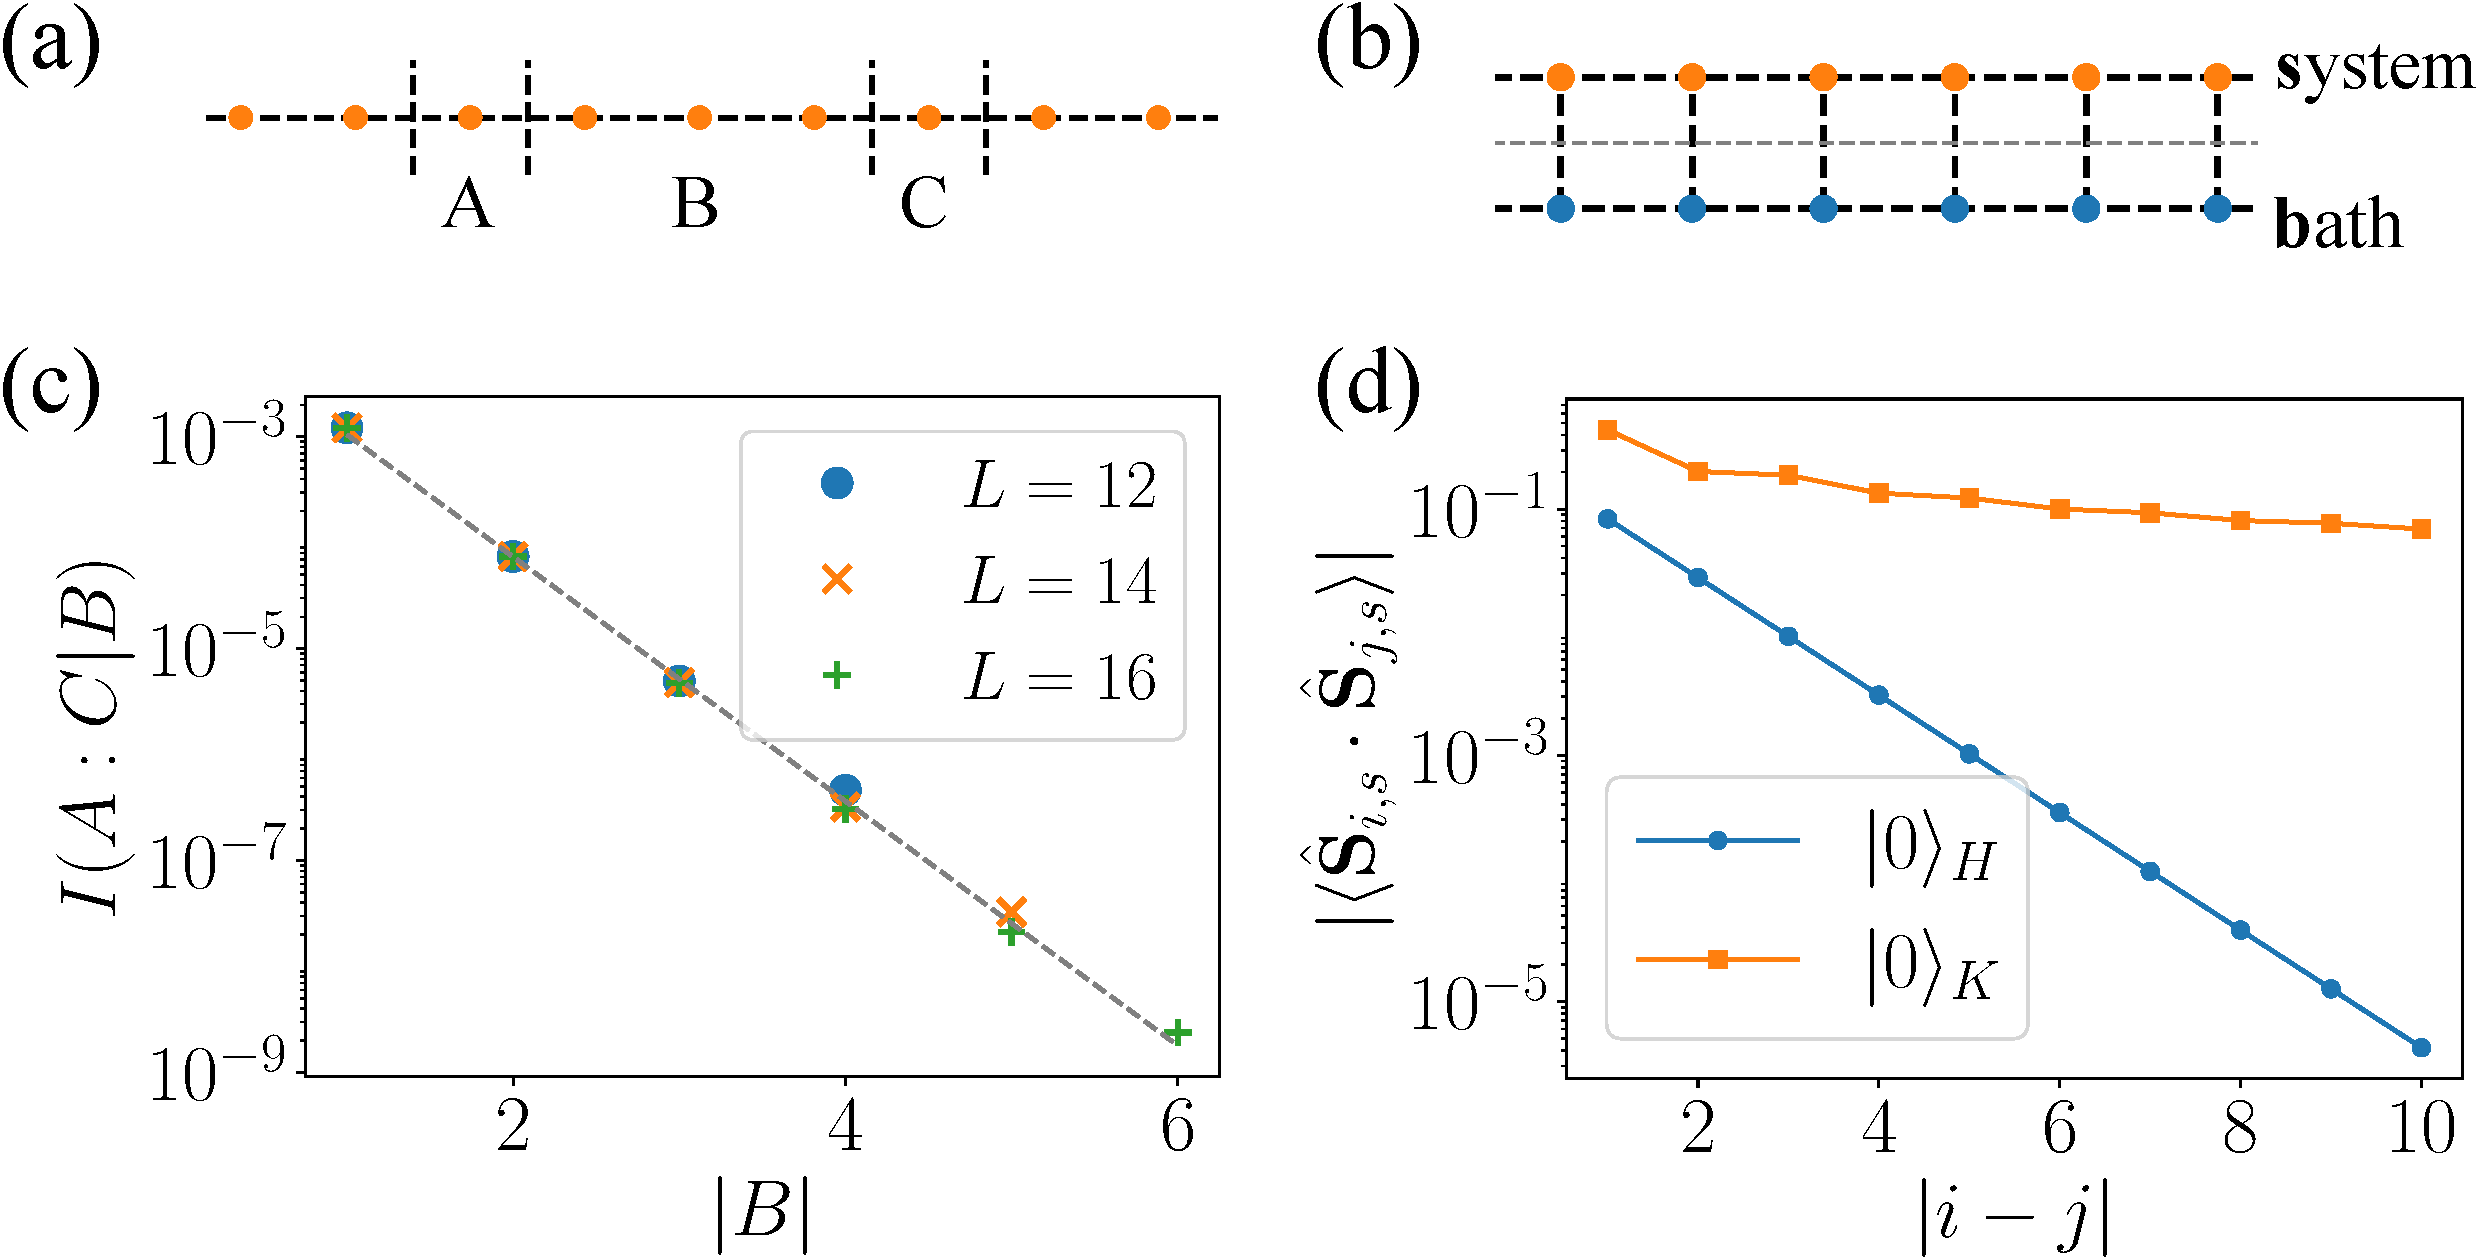
\includegraphics[width = 0.6\textwidth]{1-fig2.pdf}
    \caption{(c) Shows the behaviour of $I(A:C|B)\sim e^{-l/\xi}$. }
    \label{numerical.f}
\end{figure}
\end{frame}
%%%%%%%%%%%%%%%%%%%%%%%%%%%%%%%%%%%%%%%%%%%%%%%%
\begin{frame}{Gapless Spectrum}
\subsection{Gapless Spectrum, Ground State Degeneracy in the Numerical Result}
The $e^{-l/\xi}$ behaviour leads to the vanishing of the entanglement spectral gap,
\begin{align*}
    \anglelr{\hat{K}}_{\mrm{twist}} - \anglelr{\hat{K}}_0 &\sim L\int_{0}^{\infty}e^{-l/\xi}\lr{1-\cos\lr{\frac{2\pi l}{L}}}\mrm{d}l \\
    &\sim \frac{4\pi^2\xi^3}{L} - \frac{16\pi^4\xi^5}{L^3}+\cdots
\end{align*}
This once again shows the importance of the locality $e^{-l/\xi}$. If the entanglement Hamiltonian is not local, $\xi\to\infty$, then the upper bound of the entanglement spectral gap is broken down.
\end{frame}
%%%%%%%%%%%%%%%%%%%%%%%%%%%%%%%%%%%%%%%%%%%%%%%%
\begin{frame}{Gapless Spectrum}
\begin{minipage}[t]{0.35\textwidth}
\begin{figure}
    \centering
    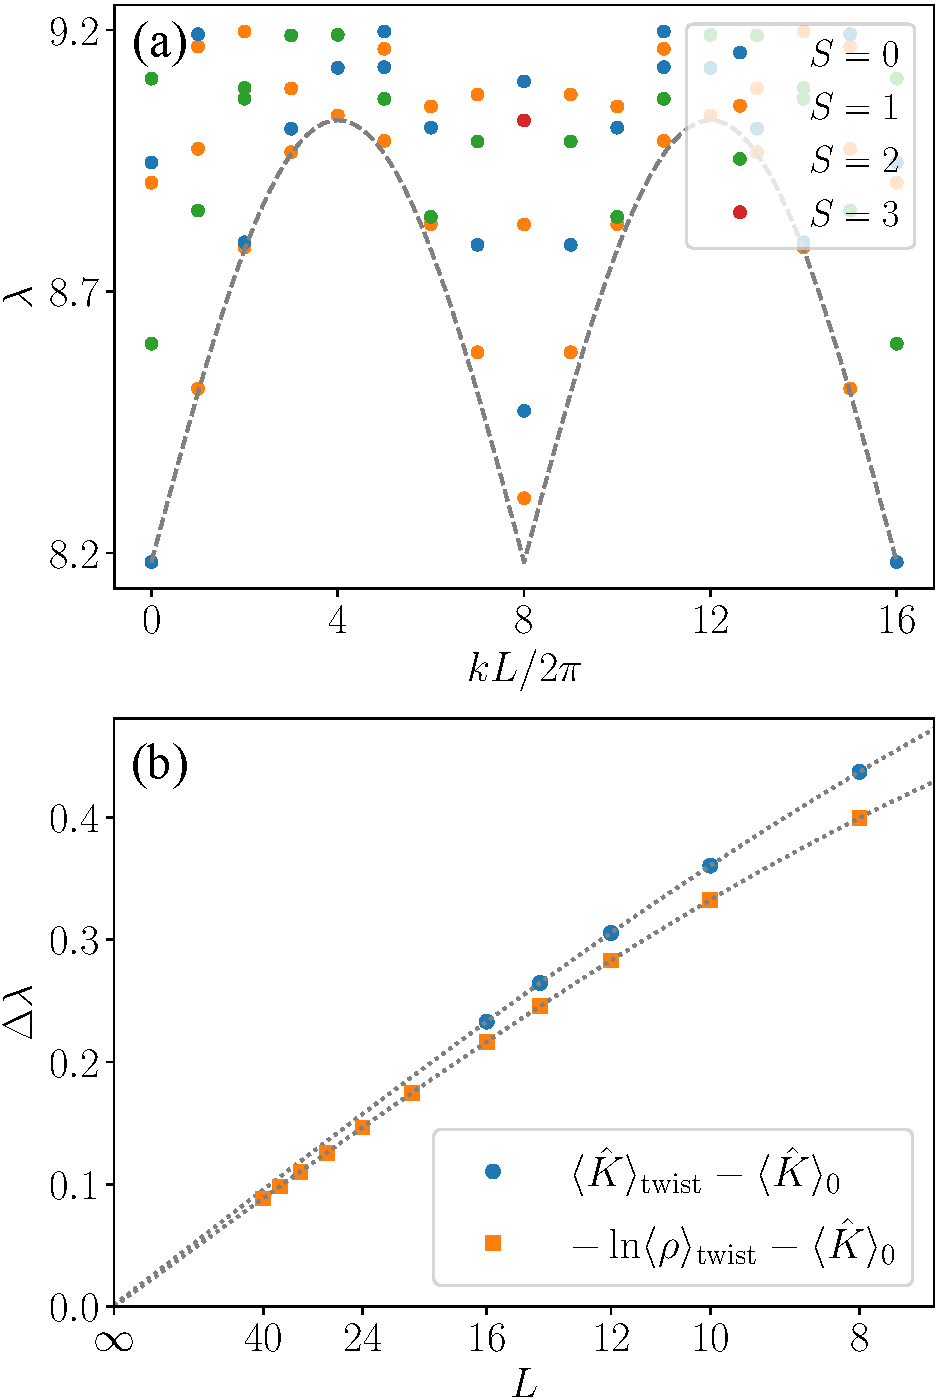
\includegraphics[width = \textwidth]{1-fig3.pdf}
    \label{gapless}
\end{figure}
\end{minipage}
\hspace{0.3cm}
\begin{minipage}[t]{0.6\textwidth}
    \begin{itemize}
        \item The upper bounds of the entanglement spectral gap:
        \begin{align*}\Delta\lambda&\leq -\ln\anglelr{\hat{\rho}}_{\mrm{twist}} - \anglelr{\hat{K}}_0 \\ &\leq\anglelr{\hat{K}}_{\mrm{twist}} - \anglelr{\hat{K}}_0\end{align*}

        \item Curve fitting: 
        \[\Delta\lambda = c_0 + c_1L^{-1} + c_3L^{-3}\]
    \end{itemize}
\end{minipage}

\end{frame}
%%%%%%%%%%%%%%%%%%%%%%%%%%%%%%%%%%%%%%%%%%%%%%%%
\begin{frame}{Ground State Degeneracy}
%\subsection{Ground State Degeneracy}
Model: Spin-1/2 Majumdar-Ghosh (MG) chain coupled to a spin-3/2 bath
{\footnotesize\[
\hat{H} = J_1\sum_{i=1}^{L}\lr{\hat{\bo{S}}_{i,s}\cdot\hat{\bo{S}}_{i+1,s} +\frac{1}{2}\hat{\bo{S}}_{i,s}\cdot\hat{\bo{S}}_{i+2,s}} + J_2\sum_{i=1}^{L}\hat{\bo{S}}_{i,s}\cdot\hat{\bo{S}}_{i,b} + D\sum_{i=1}^{L}\lr{\hat{S}^z_{i,s}+\hat{S}^z_{i,b}}^2
\]}
\begin{figure}[H]
    \centering
    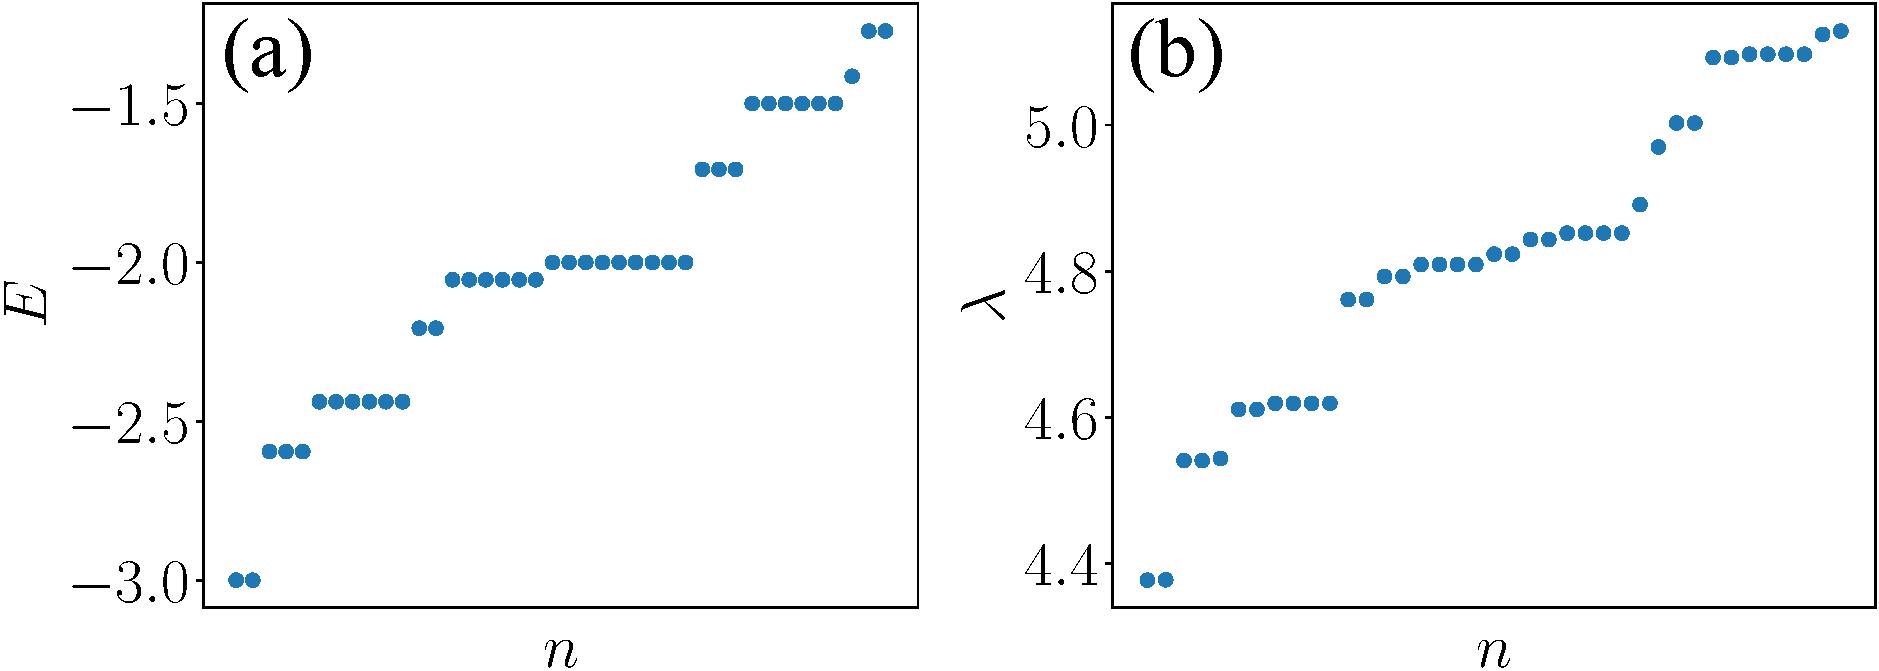
\includegraphics[width = 0.7\textwidth]{1-fig4.pdf}
    \caption{(a) The energy spectrum of a closed system (b) The entanglement spectrum. The two-fold ground state degeneracy is observed.}
    \label{gnd degeneracy.f}
\end{figure}
\end{frame}
%%%%%%%%%%%%%%%%%%%%%%%%%%%%%%%%%%%%%%%%%%%%%%%%
\begin{frame}{Questions}
%\subsection{Questions}
Here I list my questions to this paper
\begin{itemize}
    \item Is the entanglement spectrum measurable?
    \item The rigorous proof of the exponential decay behaviour of the mutual information, i.e. the quantum approximate Markov state.
\end{itemize}
\end{frame}
%%%%%%%%%%%%%%%%%%%%%%%%%%%%%%%%%%%%%%%%%%%%%%%%
%
% the next paper
%
%%%%%%%%%%%%%%%%%%%%%%%%%%%%%%%%%%%%%%%%%%%%%%%%
\begin{frame}
    \centering
\section{Literature 2}
{\Huge Literature 2}

{\Large \textit{Phys. Rev. Lett.} \textbf{132}, 070402 (2024)
}
\end{frame}
%%%%%%%%%%%%%%%%%%%%%%%%%%%%%%%%%%%%%%%%%%%%%%%%
\begin{frame}{Lindblad Equation and Dissipative Gap}
\subsection{Lindblad Equation and Dissipative Gap}

{\textbf{Motivation}}: Open quantum systems are no longer described by Hamiltonians, but instead by \textbf{Liouvillians}.

\vspace{0.3cm}

The master equation describing the evolution of the density matrix is the \textbf{Lindblad equation}
\[\dif{t}\hat{\rho}_s = \mathcal{L}\hat{\rho}_s = -i[\hat{H},\rho_s] + \sum_{n}\lrm{\hat{L}_n\hat{\rho}\hat{L}^\dagger_n - \frac{1}{2}\{\hat{L}^\dagger_n\hat{L}_n,\hat{\rho}\}}\]
$\mathcal{L}$ is called the \textit{Lindbladian}

\vspace{0.3cm}

\textbf{Question}: If we can find a quantity in a open quantum system playing the similar role as the spectral gap in the LSM theorem? 
\end{frame}
%%%%%%%%%%%%%%%%%%%%%%%%%%%%%%%%%%%%%%%%%%%%%%%%
\begin{frame}{Lindblad Equation and Dissipative Gap}

The answer given by the authors is the \textbf{dissipative gap} $\Delta$, which is the negative real part of the eigenvalue of the Lindbladian of the first decaying state.

\vspace{0.2cm}

{\footnotesize
A simple comprehension: From the lindblad equation, we have 
\[\hat{\rho}_s(t) = e^{t\mathcal{L}}\hat{\rho}_s(0)\]
If $\hat{\rho}_s(0)$ is an eigenvector of $\mathcal{L}$ with eigenvalue $iE-\Delta$, then it leads to
\[\hat{\rho}_s \sim e^{-t \Delta }\]
indicating the dissipating behaviour ($\Delta^{-1}$ is the relaxation time scale). 
}

\vspace{0.5cm}

{\tiny
References
\begin{itemize}
    \item \textit{Phys. Rev. Lett.} \textbf{111}, 150403 (2013)
    \item \textit{Phys. Rev. E} \textbf{92}, 042143 (2015)
    \item \textit{Phys. Rev. A} \textbf{107}, 033332 (2023)
    \item \textit{The Theory of Open Quantum Systems}, Oxford University Press
\end{itemize}}
    
\end{frame}
%%%%%%%%%%%%%%%%%%%%%%%%%%%%%%%%%%%%%%%%%%%%%%%%
\begin{frame}{LSM Theorem in Open Quantum Systems}

Mapping: $\hat{\rho} = \sum_{ij}\rho_{ij}\ket{i}\bra{j}\mapsto \ket{\rho} = \sum_{ij}\rho_{ij}\ket{i}_+\ket{j}_-\in \mathcal{H}=\mathcal{H}_+\otimes\mathcal{H}_-$
\vspace{0.1cm}
{\footnotesize\[\mathcal{L} = -i\hat{H}_+ + i\hat{H}_- + \sum_{n}\lrm{\hat{L}_{n,+}\hat{L}^*_{n,-} - \frac{1}{2}\lr{L^\dagger_{n,+}\hat{L}_{n,+} + \hat{L}^T_{n,-}L^*_{n,-}}}\]}

so now the Lindbladian becomes $\mathcal{L}:\mathcal{H}\to\mathcal{H}$


\vspace{0.3cm}

\textbf{Goal}: \textbf{Constraint} the steady state ($\mathcal{L}\hat{\rho}=0$) and the dissipative gap solely by \textbf{symmetry}.

\begin{itemize}
    \item Lattice translational symmetry $\mathcal{T}$
    \item $\mrm{U(1)}$ symmetry 
\end{itemize}

\vspace{0.3cm}

The conserved quantity corresponding to the $\mrm{U(1)}$ symmetry is the $N_{\pm}$

The \textbf{filling number} is defined by $\nu := N_{\pm}/V$, where $V$ is the system size (here we focus on the subspace with $N_+ = N_-$)

\end{frame}
%%%%%%%%%%%%%%%%%%%%%%%%%%%%%%%%%%%%%%%%%%%%%%%%
\begin{frame}{LSM Theorem in Open Quantum Systems}
\begin{theorem}
    In open quantum systems with \textbf{lattice translation invariance} and \textbf{strong $\mrm{U(1)}$ symmetry}, if the Lindbladian is gapped and exhibits a unique steady state in the subspace with the fixed $\mrm{U(1)}$ charge, the filling number $\nu$ is required to be an integer.
\end{theorem}
In other words, if $\nu$ is not an integer, the Lindbladian is gapless or exhibits degenerate steady states.
\end{frame}
%%%%%%%%%%%%%%%%%%%%%%%%%%%%%%%%%%%%%%%%%%%%%%%%
\begin{frame}{LSM Theorem in Open Quantum Systems}
    Twist Operator: $U^{(\mrm{twist})}_\pm := e^{2\pi i \sum_{j=1}^{L}jn_{j,\pm}/L}$ (which is equivalent to $\mrm{U(1)}$ flux insertion)
    \[\mathcal{T}U_+^{(\mrm{twist})}\mathcal{T}^{-1} = e^{-2\pi i N_+/L}U_+^{(\mrm{twist})} = e^{-2\pi i \nu}U_+^{(\mrm{twist})}\]
    Spin version: $U^{(\mrm{twist})}_\pm := e^{2\pi i \sum_{j=1}^{L}jS^z_{j,\pm}/L}$
    \[\mathcal{T}U_+^{(\mrm{twist})}\mathcal{T}^{-1} = e^{2\pi iS_1^z-2\pi i S_+/L}U_+^{(\mrm{twist})} = e^{-2\pi i (S+S_+/L)}U_+^{(\mrm{twist})}\]
    So the filling number for spin systems is defined by $\nu = S + S_\pm/L$
    \vspace{0.2cm}
 
\end{frame}
%%%%%%%%%%%%%%%%%%%%%%%%%%%%%%%%%%%%%%%%%%%%%%%%
\begin{frame}{LSM Theorem in Open Quantum Systems}
    \here $[\mathcal{T},U^{(\mrm{twist})}_\pm]=0$ only when $\nu\in\mathbb{Z}$. Otherwise, one can use $U^{(\mrm{twist})}_\pm$ to construct another state $\ket{\psi'} = U^{(\mrm{twist})}_\pm\ket{\psi}$ that is orthogonal to the original $\ket{\psi}$.

    \vspace{0.3cm}
    Consider a steady state $\ket{\rho_0}$. If $\nu\notin\mathbb{Z}$, there exists another steady state $\ket{\rho'_0} = U^{(\mrm{twist})}_+\ket{\rho_0}$\alert{?} However, since $U^{(\mrm{twist})}_\pm$ is equivalent to $\mrm{U(1)}$ gauge flux insertion (twist the boundary condition), the Lindblad gap shouldn't be opened or closed by such an operation.
    
    \vspace{0.3cm}
    \textbf{Conclusion}: The gapped Lindbladian with the unique steady state requires the integer filling number.
\end{frame}
%%%%%%%%%%%%%%%%%%%%%%%%%%%%%%%%%%%%%%%%%%%%%%%%
\begin{frame}{Numerical Result}
\subsection{Numerical Result}
{\footnotesize
\[\hat{H} = \sum_{n=1}^{L}\lrm{J\lr{S^x_{n}S^x_{n+1} + S^y_{n}S^y_{n+1}} + J_zS^z_{n}S^z_{n+1}}\]
\[\hat{L}_n = \sqrt{\gamma}S^z_n\]
This system respects $\mrm{U(1)}$ symmetry ($U_{\pm} = e^{i\theta S^z_\pm}$), $[\mathcal{L},S^z_\pm] = 0$. Thus the conserved quantity is the total $z$-magnetization $S^z:=\sum_{n=1}^{L}S^z_{n,\pm}$, and the filling number is $\nu = S^z_\pm/L + S$.
}
\begin{figure}[H]
    \centering
    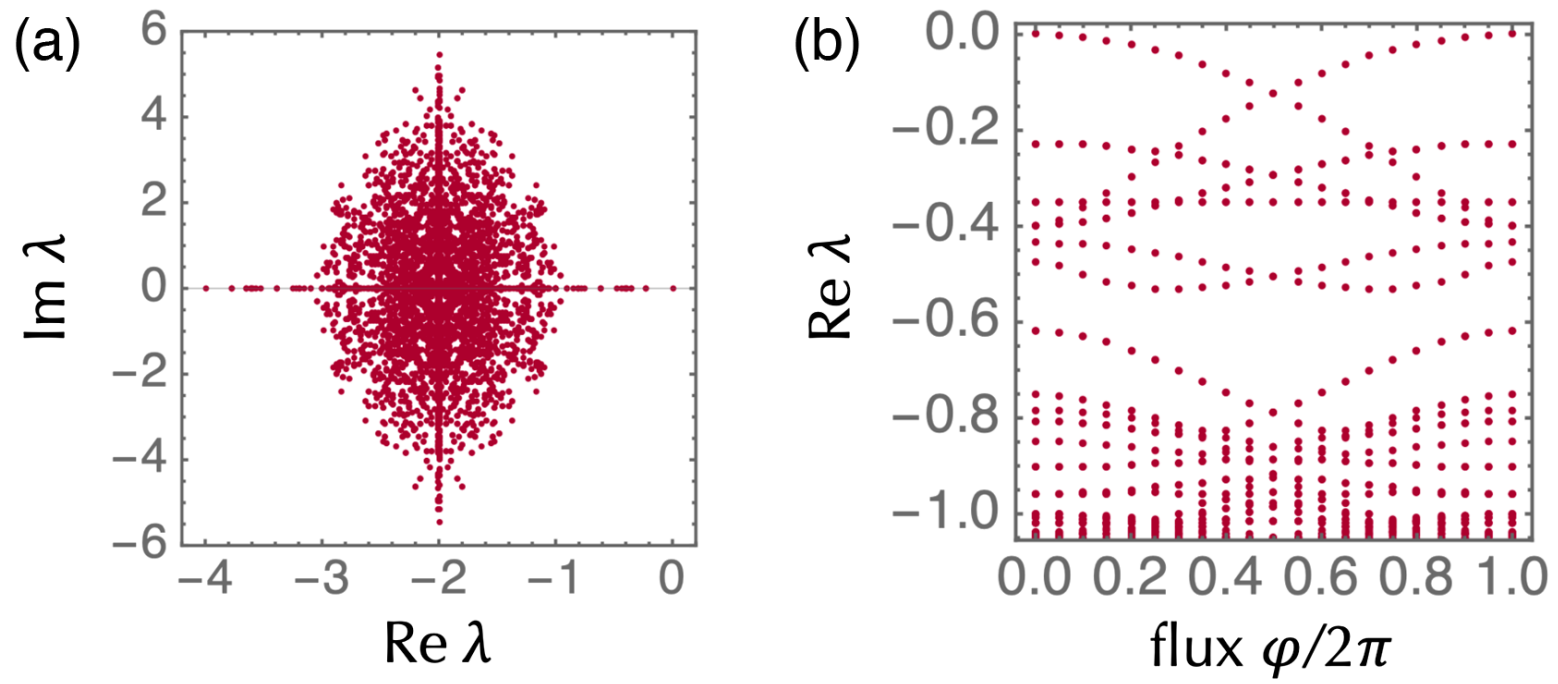
\includegraphics[height = 0.25\textheight]{Lindblad_Heisenberg_ab.png}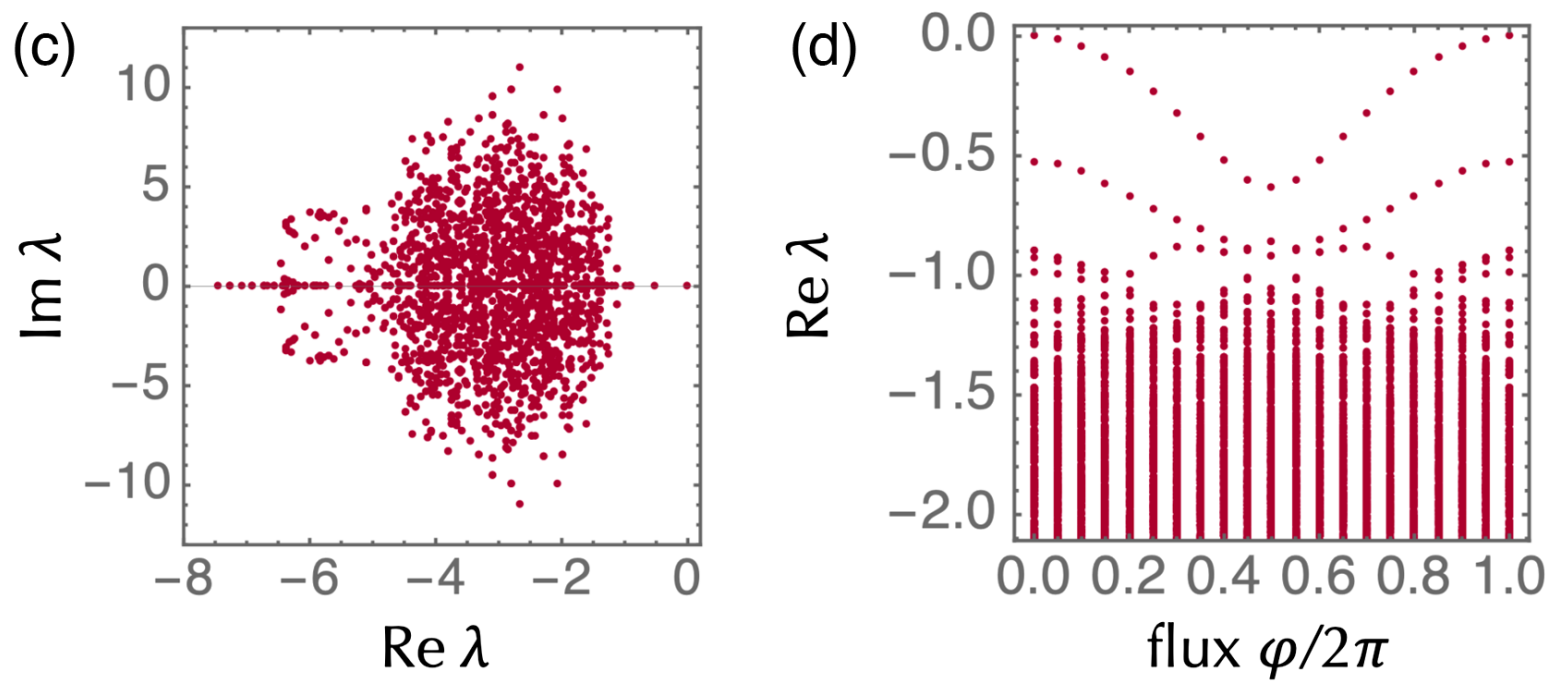
\includegraphics[height = 0.25\textheight]{Lindblad_Heisenberg_cd.png}
    \caption{Dissipative Heisenberg XXZ model with $J=J_z=\gamma = 1.0$. (a)(b) spin-1/2, $L=8$, (c)(d) spin-1, $L=5$. Here the authors set $S^z_\pm=0$ (no net magnetization)}
    \label{gapped and gapless.f}
\end{figure}
\end{frame}
%%%%%%%%%%%%%%%%%%%%%%%%%%%%%%%%%%%%%%%%%%%%%%%%
\begin{frame}{Symmetry Anomaly}
\subsection{Symmetry Anomaly}
    
\end{frame}
%%%%%%%%%%%%%%%%%%%%%%%%%%%%%%%%%%%%%%%%%%%%%%%%
\begin{frame}{Conclusion}
\section{Conclusion}
\begin{itemize}
    \item The energy spectrum is not well defined in \textbf{open quantum systems}, and the system is better described by the Lindblad equation instead of the Schr\"odinger equation for closed systems.
    \item The LSM theorem is still applicable in open quantum systems but the spectral gap should be replaced by the \textbf{entanglement spectral gap} or the \textbf{dissipative gap}.
    \item Other phenomena related to LSM theorem, e.g. the symmetry anomaly, can also be discussed in these theoretical frameworks.
\end{itemize}
\end{frame}
%%%%%%%%%%%%%%%%%%%%%%%%%%%%%%%%%%%%%%%%%%%%%%%%
\begin{frame}
\centering
\Huge
    \textsc{Thanks for Listening}
\end{frame}
%%%%%%%%%%%%%%%%%%%%%%%%%%%%%%%%%%%%%%%%%%%%%%%%
% The general question I was thinking is the possibility of unifying the two works, i.e. the entanglement spectrum gap and the dissipative gap.
%%%%%%%%%%%%%%%%%%%%%%%%%%%%%%%%%%%%%%%%%%%%%%%%
\appendix
%%%%%%%%%%%%%%%%%%% appendix %%%%%%%%%%%%%%%%%%%
\begin{frame}{Gauge transformation and twist operator}
\section{Gauge transformation and twist operator}

References:
\begin{itemize}
    \item \textit{Phys. Rev. Lett.} \textbf{78}, 1984 (1997)
    \item \emph{Phys. Rev. Lett.} \textbf{84}, 1535 (1999)
\end{itemize}
\end{frame}
%%%%%%%%%%%%%%%%%%%%%%%%%%%%%%%%%%%%%%%%%%%%%%%%

\end{document}